\section{神经网络对照与训练曲线}

在介绍完短时 FFT 模板方法和基于 AI 的重实现方法之后，本节进一步用 MLP 和 CNN 作为神经网络对照。它们都使用同一份数据划分：训练集用于参数学习，验证集用于阈值选择或早停，测试集只用于最终评测，最后统一用 $\arg\max$ 解码。

\subsection{MLP：MFCC 与频带统计特征}

MLP 的输入不是整张谱图，而是人工统计特征。对每条语音先计算 log-mel，再取 13 维 MFCC 及其一阶差分。特征向量由五部分拼接：
\[
z_i=
\left[
\mathrm{mean}(\mathrm{MFCC}),
\mathrm{std}(\mathrm{MFCC}),
\mathrm{mean}(\Delta\mathrm{MFCC}),
\mathrm{std}(\Delta\mathrm{MFCC}),
\mathrm{bandEnergy}
\right].
\]
前四部分共 $13\times4=52$ 维，最后的 band-energy 使用 10 个频带，所以 $z_i\in\mathbb{R}^{62}$。训练前先用 train 集均值和方差做标准化。

模型结构是两层隐藏层的前馈网络：
\[
h_1=\mathrm{ReLU}(W_1z_i+b_1),\qquad
h_2=\mathrm{ReLU}(W_2h_1+b_2),\qquad
p_i=\sigma(W_3h_2+b_3),
\]
隐藏层宽度为 $128$ 和 $64$。训练目标可以写成四个标签的二元交叉熵加 $L_2$ 正则：
\[
\mathcal{L}_{\mathrm{MLP}}
=-\sum_{i,c}\left[y_{i,c}\log p_{i,c}+(1-y_{i,c})\log(1-p_{i,c})\right]
+\lambda\|\theta\|_2^2.
\]
这个模型的假设是：整词级 MFCC 统计已经能保留足够的平均声学差异。它不显式定位词首，因此如果词尾元音或说话人差异占了更大比例，模型会把这些全局变化一起带进去。伪代码见附录算法~\ref{alg:mlp-ai}。

\subsection{CNN：整词 log-mel 谱图}

CNN 直接使用整词 log-mel spectrogram。设输入矩阵为 $L_i\in\mathbb{R}^{T\times40}$，先用 train 集的全局均值和标准差标准化，然后作为单通道图像输入。网络结构为
\[
\mathrm{Conv}(1,24)\rightarrow \mathrm{BN}\rightarrow \mathrm{ReLU}\rightarrow \mathrm{MaxPool},
\]
\[
\mathrm{Conv}(24,48)\rightarrow \mathrm{BN}\rightarrow \mathrm{ReLU}\rightarrow \mathrm{MaxPool},
\]
\[
\mathrm{Conv}(48,96)\rightarrow \mathrm{BN}\rightarrow \mathrm{ReLU}\rightarrow
\mathrm{GlobalAvgPool}\rightarrow \mathrm{FC}(96)\rightarrow \mathrm{Dropout}(0.25)\rightarrow \mathrm{FC}(4).
\]
输出 logits 记为 $u_{i,c}$，概率为 $p_{i,c}=\sigma(u_{i,c})$。训练损失使用带正样本权重的 binary cross entropy：
\[
\mathcal{L}_{\mathrm{CNN}}
=-\sum_{i,c}\alpha_c y_{i,c}\log p_{i,c}
-(1-y_{i,c})\log(1-p_{i,c}),
\]
其中 $\alpha_c$ 由 train 集正负样本比例得到，并限制在 $[1,10]$。优化器是 AdamW，学习率 $10^{-3}$，weight decay 为 $10^{-4}$，并用 dev macro-F1 选择最佳 epoch。

CNN 的假设和模板法不同。它不预先规定词首窗口，而是希望卷积核从整词谱图里学到局部模式。这个假设需要更多词表覆盖支撑；扩大到 300 个词、6796 条语音后，小 CNN 的表现明显好于 60 词版本。

\begin{table}[H]
    \centering
    \caption{神经网络对照的整体指标}
    \label{tab:ai-summary}
    \begin{tabular}{lccccc}
        \toprule
        方法 & label-wise acc. & exact-match acc. & macro-F1 & micro-F1 & samples-F1 \\
        \midrule
        MLP & 0.7423 & 0.4845 & 0.4848 & 0.4845 & 0.4845 \\
        CNN & 0.7796 & 0.5593 & 0.5557 & 0.5593 & 0.5593 \\
        \bottomrule
    \end{tabular}
\end{table}

从结果上看，MLP 是一个稳定的统计基线，但仍低于基于 AI 的重实现方法。CNN 受益于更多词种和更多训练样本，exact-match 达到 0.559，高于基于 AI 的重实现方法的 0.503。这说明在词表覆盖扩大之后，端到端谱图模型开始能够学到一部分词首局部模式，但它的解释性仍弱于模板方法。

\begin{table}[H]
    \centering
    \caption{CNN epoch 消融结果}
    \label{tab:epoch-ablation}
    \begin{tabular}{ccccc}
        \toprule
        最大 epoch & 实际完成 & dev 最优 epoch & dev macro-F1 & test exact-match \\
        \midrule
        5 & 5 & 5 & 0.529 & 0.372 \\
        10 & 10 & 8 & 0.575 & 0.499 \\
        15 & 15 & 11 & 0.598 & 0.460 \\
        20 & 20 & 18 & 0.598 & 0.523 \\
        25 & 25 & 25 & 0.608 & 0.559 \\
        30 & 30 & 26 & 0.614 & 0.541 \\
        40 & 34 & 26 & 0.614 & 0.541 \\
        \bottomrule
    \end{tabular}
\end{table}

按 dev macro-F1 看，30 和 40 的上限都能找到第 26 个 epoch 附近的最优点；但 40 会在 34 个 epoch 早停，没有带来新收益。按测试集 exact-match 看，25 个 epoch 的设置最高。因此，正文采用 25 个 epoch 作为最终 CNN 配置，并把 25--30 视为这个数据规模下较为合适的训练区间。

\begin{figure}[H]
    \centering
    
\includegraphics[width=0.92\textwidth]{figures/mswc_course_gbdz_75w_cap40_5_5/cnn_history.png}
    \caption{CNN 的训练曲线。}
    \label{fig:cnn-history}
\end{figure}

\begin{figure}[H]
    \centering
    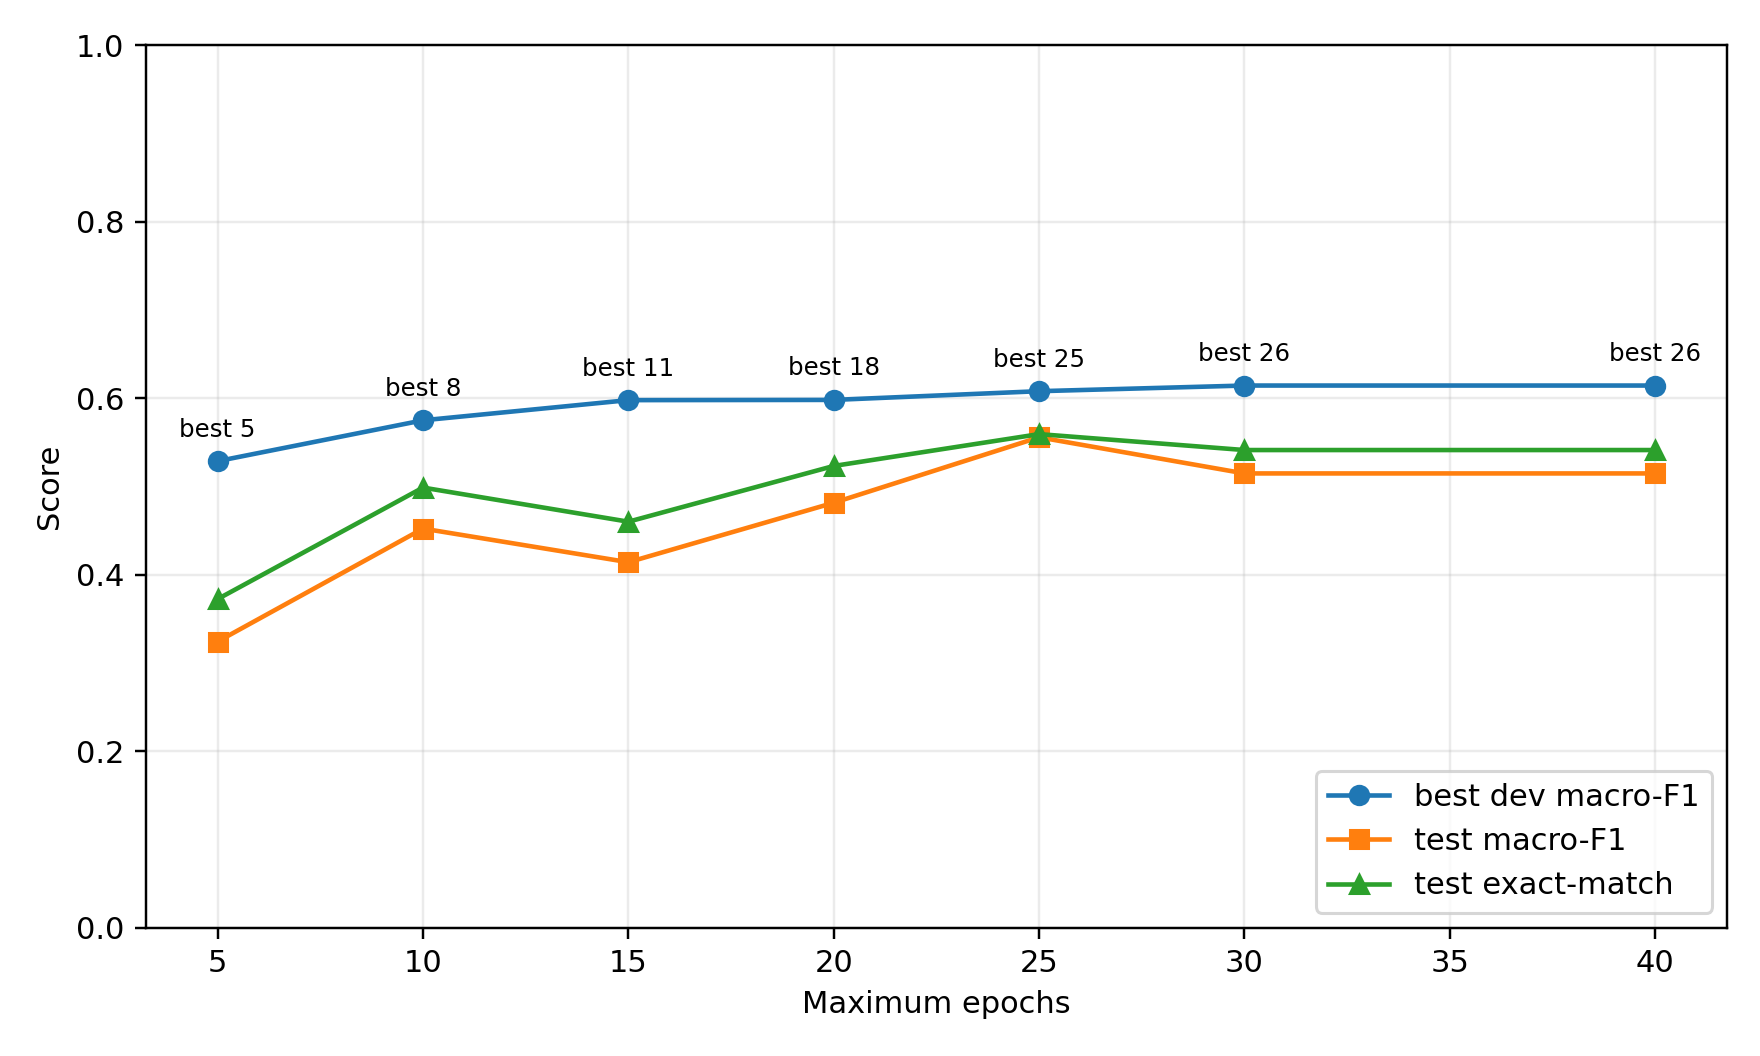
\includegraphics[width=0.86\textwidth]{figures/mswc_course_gbdz_75w_cap40_5_5/cnn_epoch_ablation.png}
    \caption{CNN 最大 epoch 消融。25 个 epoch 的测试 exact-match 最高，30/40 的 dev macro-F1 略高，但测试集没有继续提升。}
    \label{fig:cnn-epoch-ablation}
\end{figure}

\begin{figure}[H]
    \centering
    
\includegraphics[width=0.92\textwidth]{figures/mswc_course_gbdz_75w_cap40_5_5/metric_summary.png}
    \caption{全部方法的总体指标汇总。}
    \label{fig:metric-summary}
\end{figure}

\begin{figure}[H]
    \centering
    
\includegraphics[width=0.92\textwidth]{figures/mswc_course_gbdz_75w_cap40_5_5/per_label_f1.png}
    \caption{全部方法在四个标签上的 F1 对比。}
    \label{fig:per-label-f1}
\end{figure}

综合来看，神经网络模型在数据规模扩大后能够进一步提高整体分数，但这种提升主要体现在判别能力上，而不是声学解释能力上。
